\documentclass{article}
\usepackage[utf8]{inputenc}
\usepackage{amsmath}
\usepackage{amsfonts}
\usepackage{amssymb}
\usepackage{graphicx}
\usepackage{geometry}
\usepackage{xcolor}
\usepackage{gensymb}
\usepackage{hyperref}
\usepackage{gensymb}
\usepackage{listings}

\newcommand{\inv}{^{-1}}
\newcommand{\Z}{\mathbb Z}
\newcommand{\R}{\mathbb R}
\newcommand{\Q}{\mathbb Q}
\newcommand{\C}{\mathbb C}
\newcommand{\N}{\mathbb N}

\begin{document}

\noindent{\bf 1.}

Since the time constant is .0002 seconds, the capacitor has time to get really close to fully charged and discharged.
\begin{center}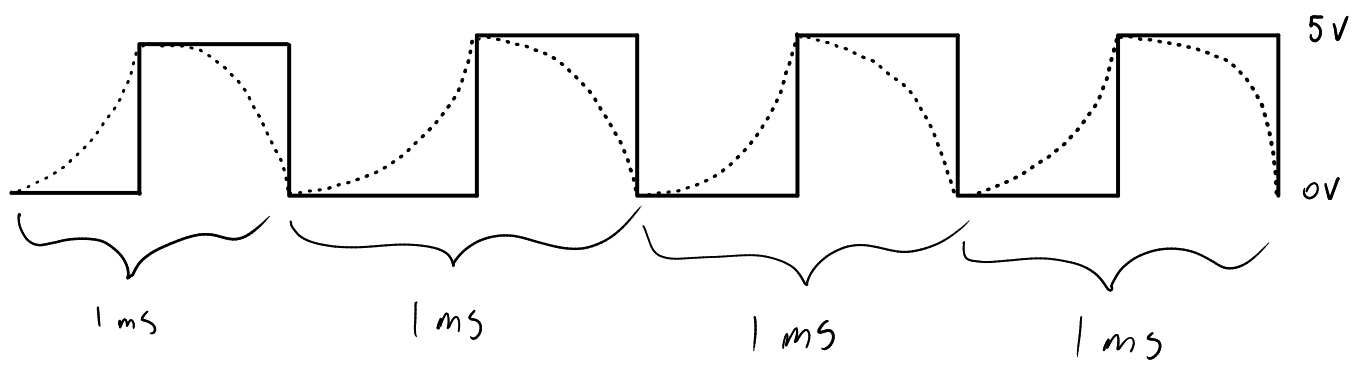
\includegraphics[scale=.4]{sharktooth.png}\end{center}

\newpage\noindent{\bf 2.}

    \begin{center}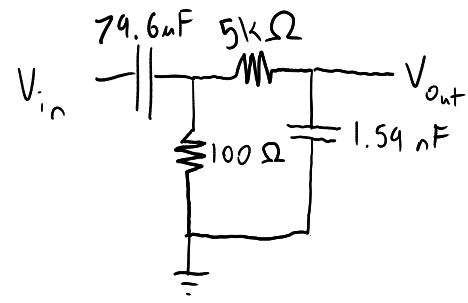
\includegraphics{bandpass.png}\end{center}

\newpage\noindent{\bf 3.}

    Since we have a 30V RMS input to the bridge rectifier, its output will be $30\sqrt2 -1.2$V P-P.
    Thus, our peak voltage is $30\sqrt2 - 1.2 \approx 41.23V.$
    Therefore, assuming our ripple voltage is negligible, our output current will be $\frac{41.23}{3400} \approx 12\text{mA}.$
    Thus, the ripple voltage is $\frac{.012}{120 \cdot 1000 \cdot 10^{-06}} = 0.1$V.

\newpage\noindent{\bf 4.}

    The voltage drop across the resistor is 8V, so the current through the resistor is 400mA.
    Thus, the drain-source current is 400mA, so the curve tells us that the gate-source voltage is about 2.95V.
    Thus, Vin is 2.95V.

\newpage\noindent{\bf 5.}

    \begin{center}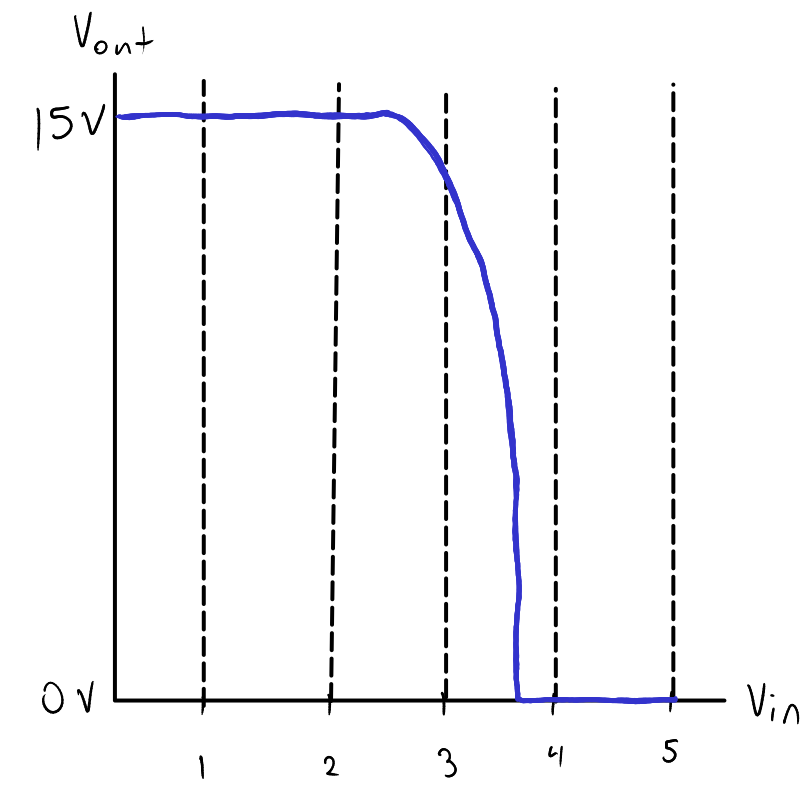
\includegraphics[scale=.5]{5.png}\end{center}

\newpage\noindent{\bf 6.}

    \textbf{a)} The voltage at point $a$ is 30V, and the voltage at point $b$ is 0V.
    
    \textbf{b)} The motor will not turn.
    
    \textbf{c)} No current is flowing through either FET.
    
    \textbf{d)} No power is dissipated in either FET.

\newpage\noindent{\bf 7.}

    \textbf{a)} The voltage at point $a$ is 0V, and the voltage at point $b$ is 30V.
    
    \textbf{b)} The motor will turn.

    \textbf{c)} There is 30mA flowing through the 2N7000, there is 750mA flowing through the IFRD9014.
    
    \textbf{d)} 

\newpage\noindent{\bf 8.}

\begin{center}\begin{tabular}{| c | c | c |}
    \hline
    A & B & Q \\
    \hline
    0 & 0 & 1 \\
    0 & 1 & 1 \\
    1 & 0 & 0 \\
    1 & 1 & 1 \\
    \hline
\end{tabular}\end{center}

$$Q = (\text{NOT } B) \text{ NAND } A.$$

\newpage\noindent{\bf 9.}

    \begin{align*}
        115 + -17 &= 0\text b01110011 +
                     0\text b11101111 \\
                  &= 0\text b01100010 \\
                  &= 98
    \end{align*}

\newpage\noindent{\bf 10.}
\begin{verbatim}i=list(iter(input,""));print(max(i),min(i))
\end{verbatim}

\end{document}
